\hypertarget{vector3d_8cpp}{\section{vector3d.\-cpp \-File \-Reference}
\label{d7/d35/vector3d_8cpp}\index{vector3d.\-cpp@{vector3d.\-cpp}}
}


\-Definition of member functions and operators of the \hyperlink{classVector3d}{\-Vector3d} class.  


{\ttfamily \#include \char`\"{}vector3d.\-h\char`\"{}}\*
\-Include dependency graph for vector3d.\-cpp\-:\nopagebreak
\begin{figure}[H]
\begin{center}
\leavevmode
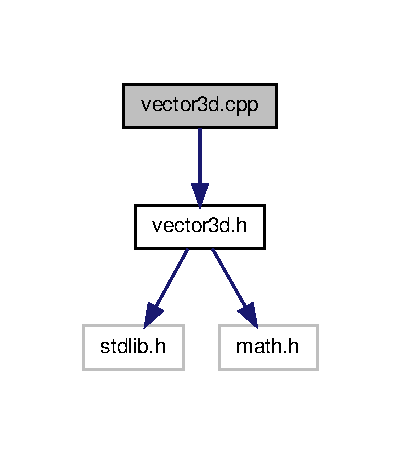
\includegraphics[width=152pt]{d5/d7b/vector3d_8cpp__incl}
\end{center}
\end{figure}


\subsection{\-Detailed \-Description}
\-Definition of member functions and operators of the \hyperlink{classVector3d}{\-Vector3d} class. \begin{DoxyAuthor}{\-Author}
\-Adhish \-Majumdar 
\end{DoxyAuthor}
\begin{DoxyVersion}{\-Version}
0.\-0 
\end{DoxyVersion}
\begin{DoxyDate}{\-Date}
22/04/2013
\end{DoxyDate}
\-This file defines the member functions and operators of the \hyperlink{classVector3d}{\-Vector3d} class representing a single 3-\/dimensional vector in the simulation. 

\-Definition in file \hyperlink{vector3d_8cpp_source}{vector3d.\-cpp}.

